\documentclass[12pt, a4paper]{ctexart} % 使用ctexart文档类,支持中文

%%%%%%%%% 页边距设置 %%%%%%%%%
\usepackage{geometry}
\usepackage{graphicx}
\usepackage[english]{babel}
\usepackage{color}
\usepackage{amsmath}
\usepackage{amssymb}
\usepackage{tcolorbox}
%\usepackage{hyperref}
\input{journal_macros.tex}
\def\tbox#1{\begin{tcolorbox}#1\end{tcolorbox}}
\geometry{a4paper, left=2.5cm, right=2.5cm, top=2.5cm, bottom=2.5cm} % 设置A4纸和页边距

%%%%%%%%% 页眉页脚设置 %%%%%%%%%
\pagestyle{headings}

%%%%%%%%% 超链接设置(使目录可点击) %%%%%%%%%
\usepackage[colorlinks, linkcolor=blue, urlcolor=blue, citecolor=blue]{hyperref}

%%%%%%%%% 文档开始 %%%%%%%%%
\begin{document}
\thispagestyle{empty}
%%%%%%%%% 标题区域 %%%%%%%%%
\title{\Huge \textbf{DroPS}  \\ \huge {\color{blue}D}eriving {\color{blue} $r$} fr{\color{blue}o}m {\color{blue}P}ower {\color{blue}S}pectra}
\author{Zhiqi Huang \\
huangzhq25@mail.sysu.edu.cn}
\date{\today} % 自动显示当前日期,若不需要可改为 \date{}
\maketitle % 生成标题

\thispagestyle{empty} % 标题页不显示页眉页脚
\newpage

%%%%%%%%% 生成目录 %%%%%%%%%
\tableofcontents
\newpage % 目录后换页

%%%%%%%%% 正文内容 %%%%%%%%%
\section{Introduction}


\subsection{Primordial power spectra}
According to the standard cosmological model, the cosmic microwave background (CMB) and the large-scale structure of the universe originated from tiny, nearly Gaussian metric fluctuations in the primordial universe. At linear order, these primordial metric fluctuations can be decomposed into scalar, vector, and tensor modes. Vector perturbations decay rapidly and are therefore generally assumed to be negligible. The primordial scalar and tensor perturbations are respectively parameterized by the dimensionless scalar power spectrum $\mathcal{P}_S(k)$ and tensor power spectrum $\mathcal{P}_T(k)$, where $k$ denotes the comoving wavenumber.

Guided by slow-roll inflation models, the primordial power spectra are commonly parameterized as
\begin{equation}
\mathcal{P}_S(k) = A_s \left(\frac{k}{k{\mathrm{pivot}}}\right)^{n_s - 1},
\end{equation}
and
\begin{equation}
\mathcal{P}_T(k) = r A_s \left(\frac{k}{k{\mathrm{pivot}}}\right)^{n_t}.
\end{equation}
The scalar amplitude $A_s$ and spectral tilt $n_s$ have been tightly constrained by CMB experiments~\cite{Planck18Params}. In most viable inflationary scenarios, the tensor tilt $n_t$ is very small; it is typically either fixed to zero or set to the slow-roll prediction $n_t = -r/8$. The tensor-to-scalar ratio $r$ at the pivot scale, however, remains poorly measured. As of this writing, the best 95\% confidence-level (CL) upper limit is $r < 0.032$~\cite{Tristram22}. Nevertheless, a broad range of inflationary models remains consistent with $0 < r < 0.032$.  

\subsection{CMB B-polarization and $r$}

The search for the signature of primordial gravitational waves in CMB, i.e., measuring $r$ from CMB is one of the most compelling pursuits in modern cosmology. This quest focuses on a unique observable: the B-mode polarization pattern.

The CMB photons became polarized when they scattered off free electrons in the early universe. This process imprinted a directional preference on the light, creating two distinct patterns: E-modes, which have a curl-free pattern like the electric field around charges, and B-modes, which have a curl-like pattern. While density fluctuations (scalar perturbations) in the primordial plasma can generate E-modes and a small amount of B-modes through gravitational lensing (so-called lensing B-modes), they cannot produce the specific, large-scale curl-like pattern of primordial B-modes.

This is where primordial gravitational waves come in. These waves, theorized to be generated during the inflationary epoch, are literally ripples in the fabric of spacetime. As they propagated through the early universe, they periodically stretched and squeezed space, imparting a unique, curl-like distortion to the plasma. This gravitational tugging created a polarization pattern in the CMB that is fundamentally rotational in nature—the primordial B-mode polarization.

Therefore, the B-mode power spectrum at large angular scales acts as a direct tracer for these primordial gravitational waves. A confident detection of this primordial B-mode signal would be tantamount to detecting the gravitational waves themselves. Its amplitude is directly proportional to the energy scale of inflation, with the tensor-to-scalar ratio $r$ quantifying the strength of the signal. Measuring this B-mode power spectrum thus provides a unique window into the physics of the universe's first moments and the grand unification of gravity and quantum mechanics.

\subsection{Ground-based CMB experiments with small-aperture telescopes}

Many ground-based CMB experiments with small-aperture telescopes (SAT), such as BICEP/Keck~\cite{BICEP}, AliCPT~\cite{AliCPT}, and Simons Observatory SAT (SO-SAT)~\cite{SO-SAT} aim to measure the CMB B-mode polarization at degree scales and to constrain the primordial gravitaional waves. These telescopes typically measure the sky emission in the range between $30\mathrm{GHz}$ and $300\mathrm{GHz}$. The raw signals measured by these telescopes are mixture of Galactic foreground, CMB, shot noise, instrumental noise, and contamination from the ground and atmoshpere. Extracting CMB B-mode polarization signal from the mixure of signals is a non-trivial problem and need to be dealt with by specialized softwares. DroPS is one of the software does this job, primarily designed for the ground-based small-aperture telescopes.

\section{Software Documentation}


\subsection{Installing DroPS}

The instruction here has been tested on Ubuntu-24.04.3LTS, and should be easily extendable to other linux platforms. A bit twists may need to be done if you are working with Windows or Mac-OS.

\subsubsection{Installing Tools and Libraries}

Install the following packages and libraries with Synaptic Package Manager (or ``sudo apt install''):

\begin{itemize}
  \item{git}
  \item{gcc}
  \item{gfortran}
  \item{cmake}
  \item{python3-pip}
  \item{python-is-python3}
  \item{python3-venv}
  \item{openmpi-dev}
  \item{libxcb-cursor0}
  \item{libcfitsio-dev}
  \item{libgsl-dev}
  \item{libfftw3-dev}
  \item{libfftw3-mpi-dev}
  \item{libhealpix-dev}
\end{itemize}

\subsubsection{Set up a python virtual environment}

Create a directory for python virtual environment in your work path (hereafter denoted as YourWorkPath)
\tbox{mkdir YourWorkPath/.work}

Create the python virtual environment
\tbox{python  -m  venv YourWorkPath/.work}

Activate the virtual environment
\tbox{source YourWorkPath/.work/bin/activate}
On windows you may need to run
\tbox{YourWorkPath/.work/Scripts/activate.bat}
in cmd.exe or
\tbox{YourWorkPath/.work/Scripts/activate.psl}
in PowerShell.

When you are done with your work, exit the terminal or use
\tbox{deactivate}
to exit the virtual environment.

If you are not working with other python projects. You may want to activate the virtual environment automatically with the terminal 
\tbox{echo ``source YourWorkPath/.work/bin/activate'' \>\> $\sim$/.bashrc}

\subsubsection{Install requirements}


Activate the virtual environment either manually or automatically as described in the previous subsection.

Upgrade pip for the latest information of packages:
\tbox{pip install -\,-upgrade pip}

Now enter your work path where you want to install DroPS
\tbox{cd YourWorkPath}
Get the DroPS repository
\tbox{git clone https://github.com/zqhuang/DroPS}

Now enter the DroPS directory
\tbox{cd DroPS}
Install all dependences
\tbox{pip install -r requirements.txt}

\subsubsection{Hack pysm3}

Hacking a python package is probably against the basic idea of python, but we are doing it anyway to improve the efficiency of CMB simulations. If you only want to analyze maps, however, you can skip this ``unpleasant'' step.

Enter the DroPS directory
\tbox{cd YourWorkPath/DroPS}
Move the cmb.py file in the pysm3 package to somewhere else
\tbox{mv PATH\_TO\_pysm3/models/cmb.py cmb\_backup.py}
and replace it with the cmb.py file that comes with DroPS
\tbox{cp cmb.py PATH\_TO\_pysm3/models/}
Here PATH\_TO\_pysm3 stands for the path where pysm3 was installed. On Ubuntu 24.04.3LTS, you may find PATH\_TO\_pysm3 to be

YourWorkPath/.work/lib/python3.12/site-packages/pysm3

If you are not using Ubuntu24.04.3LTS, the pysm3 path may be slightly different. You can find out the path by doing
\tbox{sudo apt install plocate}
and
\tbox{locate pysm3}


\subsection{Base simulations}

\subsubsection{Generate a TOD filtering model}

A critical step in processing data from ground-based CMB experiments is the removal of contaminating ground and atmospheric signals from the time-ordered data (TOD). To simulate this filtering, one needs specific information about the experiment's site, which is not currently available. Fortunately, the overall effect of the filtering is understood: it suppresses large-scale (low multipole) power in the resulting maps and introduces non-Gaussianity by mixing different Fourier modes.

If you are not keen about simulating precise filtering effect for a specific experiment, you may use the ``mock filtering'' tool that comes with DroPS to generate a filtering matrix:
\tbox{python mock\_filtering.py}

Follow the prompt and enter the healpix resolution (nside, 128 for testing, 256/512 for serious simulations) and the file name for the filtering matrix (e.g. filter\_128.pickle).


\subsubsection{Base simulations}

In this section, we run ``base simulations'' to obtain the statistics of the sky.

To begin with, you can simulate noise/cmb/foreground maps with a 4-channel ground-based experiment
\tbox{python simulate.py Test/test\_sim\_config.txt}
Read the configuration file Test/test\_sim\_config.txt to understand how the experiment is specified.

In this step, you generate a lot of noise and CMB maps based on the noise model and cosmology that are specified in the configuration file.

You also generate a foreground map in this step, based on the model ['d0', 's0'] that is specified in the configuration file. We are not able to generate ``a lot of foreground maps'', as we do not really understand the details of the statistics of the Galactic emission. This ['d0', 's0'] foreground map only captures the gross feature of the Galactic emission. The ``actual foreground'' that we will analyze in the next section can be different from the one in the base simulations.

To understand what ['d0', 's0'] means. Follow the pysm3 documentation at \url{https://pysm3.readthedocs.io/}.

\subsection{Analyzing the sky maps}

In the last section, we run ``base simulations'' based on the known noise model, assumed foreground model (['d0', 's0'])  and some assumed $r$ values. In this section, we simulate the ``observed sky'' with the same noise model, optionally a different foreground model, and a $r$ value that has nothing to do with the base simulations. DroPS will reconstruct $r$ by comparing the ``observed sky'' with  the base simulations.

\subsubsection{Analyzing one realization of sky}

Generate the ``observed sky'' with, e.g.,
\tbox{python simulate.py Test/test\_sim\_config.txt maps/test\_  0.01 999}

You can replace maps/test\_ with your preferred prefix for the output maps, 0.01 with your preferred fiducial r, and 999 with your preferred random seed. To test whether DroPS can deal with a spatial variation of the foreground, you may also replace the ['d0', 's0'] foreground model with ['d1', 's1'] in the configuration file Test/test\_sim\_config.txt.

Now analyze the ``observed sky'' with
\tbox{python mainpipe.py Test/test\_ana\_config.txt maps/test\_}
Read the configuration file Test/test\_ana\_config.txt to understand how to analyze the maps with different settings.

\subsubsection{Analyzing multiple realizations of sky}

In this step we will simulate the sky with may different random seeds, and anlyze all the simulations. The purpose is to test whether the measured $r$ is biased or not.

First you clean up the log file for $r$:
\tbox{rm Test/r\_logfile.txt}
This time we choose a different foreground model [``d1'', ``s1''] (modify Test/test\_sim\_config.txt). Now run the simulations and analyze them by running the following shell script
\tbox{./test\_bias.sh}
Plot the result
\tbox{python utils/plot\_rs.py Test/r\_logfile.txt 0.01}
Here $0.01$ is the fiducial value of $r$ used in simulations (see sim.sh). The ``mean of mean'' is supposed to be very close to the fiducial value, as shown in Figure~\ref{fig:r_logs}.
\begin{figure}
  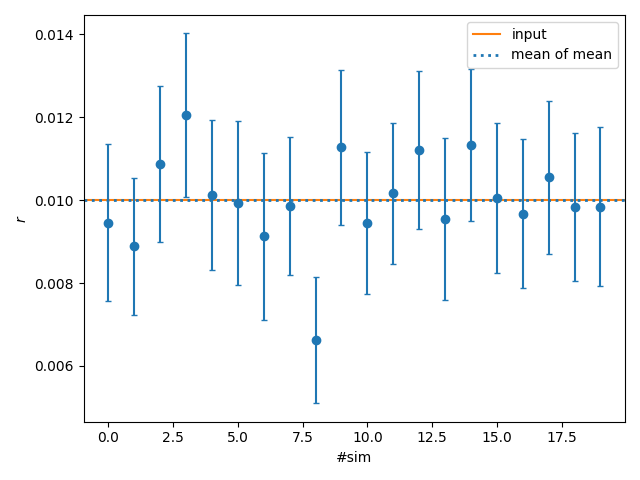
\includegraphics[width=\textwidth]{r_logs.png}
  \caption{Reconstructed $r$ for 20 skys with different random seeds. For each sky, the $r$ value is reconstructed by comparing the sky with 300 simulations. The 20 skys are simulated with foreground model ['d1','s1'] (spatially varying SED of synchrotron and dust emission), while  ['d0', 's0'] (fixed SED) is used in the 300 simulations. \label{fig:r_logs}}
\end{figure}


\subsubsection{How to apply on real data}

A real experiment comes with its own pipeline of noise simulations and TOD filtering, and provides the actually observed sky maps. To analyze the real data, you can simply replace the base simulations with the maps from the simulation pipeline of the experiment, and replace the simulated sky maps with the actually observed ones.


\subsubsection{Comparing with other pipelines}

DroPS has been applied on AliCPT data challenge (simulated 14\% sky, 95GHz and 150GHz) and achieved consistent results with other methods~\cite{Zhang24}. Here we further compare DroPS with three pipelines that have been applied on simulation data of SO-SAT (Wolz et al. 2024~\cite{SO-SAT}). We adopt the optimistic configuration of SO-SAT. The input fiducial $r$ is zero, and in the analyses nonphysical negative $r$ is allowed\footnote{in DroPS this is realized by setting r\_lowerbound negative in the configuration file}.  The results are shown in Figure~\ref{fig:compare_SO}.  From top to bottom, foreground models ``d0, s0'', ``d1, s1'', and ``dm, sm'' are used, respectively. From the left where the reconstructed mean values of $r$ and the bias (mean of the mean values of $r$) are shown, we find DroPS has negligible biases for all cases and more stable than the three pipelines tested in Wolz et al. The right column shows $\sigma_r$, the statistical uncertainties in $r$. We again find good consistency between DroPS and the other pipelines.

\begin{figure}
  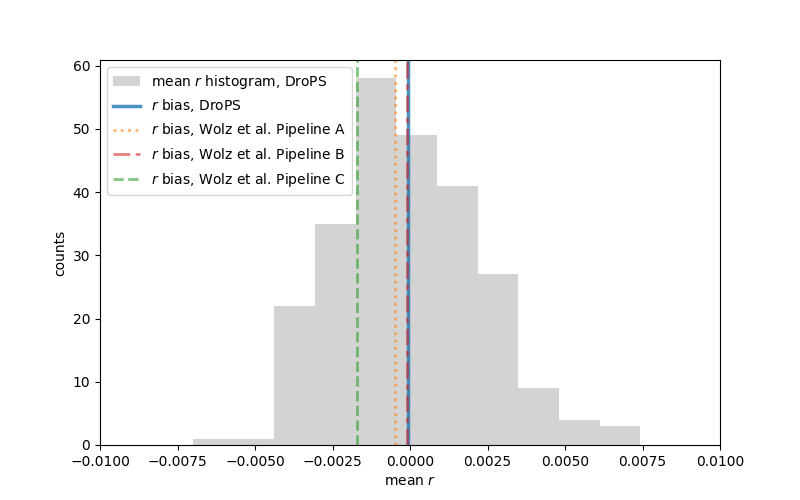
\includegraphics[width=0.5\textwidth]{d0s0_mean.png}%
  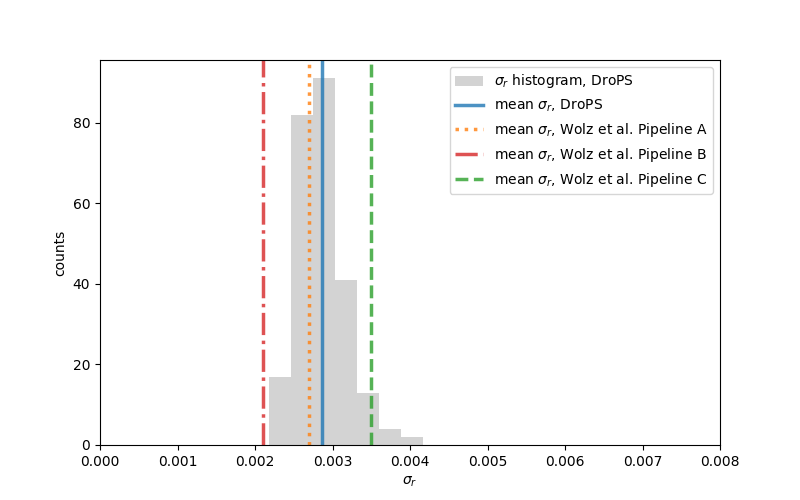
\includegraphics[width=0.5\textwidth]{d0s0_std.png}
  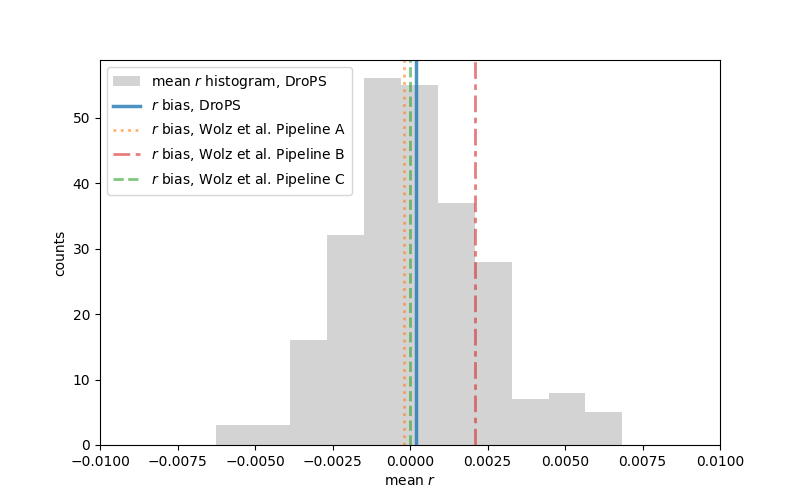
\includegraphics[width=0.5\textwidth]{d1s1_mean.png}%
  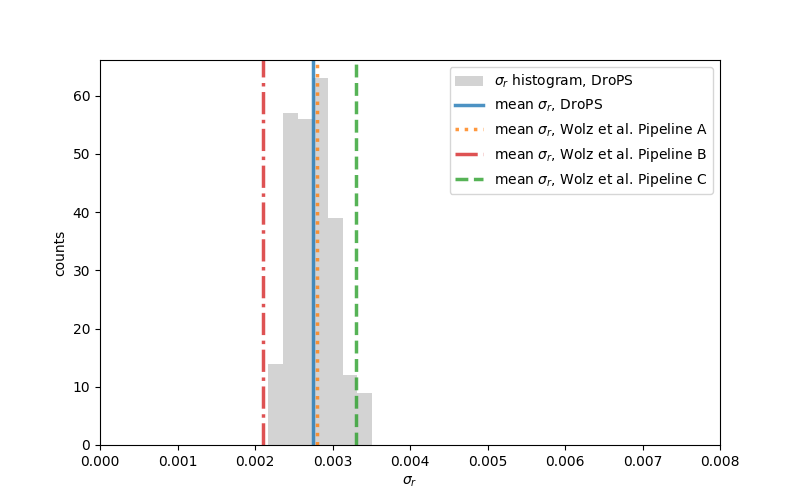
\includegraphics[width=0.5\textwidth]{d1s1_std.png}
  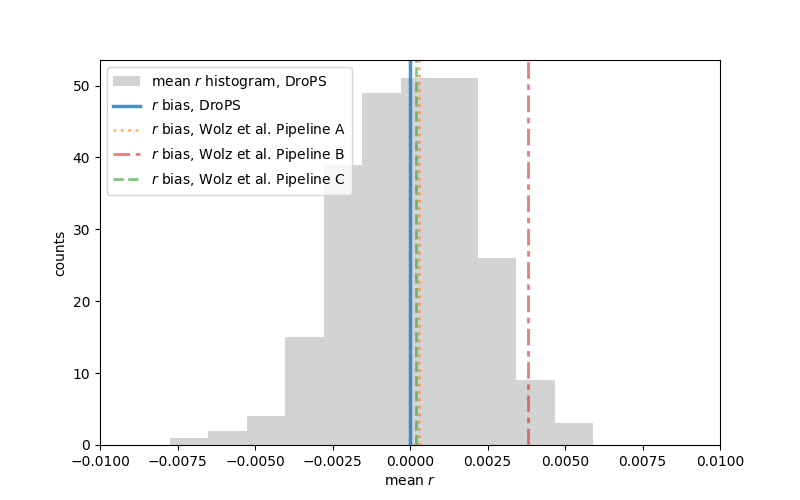
\includegraphics[width=0.5\textwidth]{dmsm_mean.png}%
  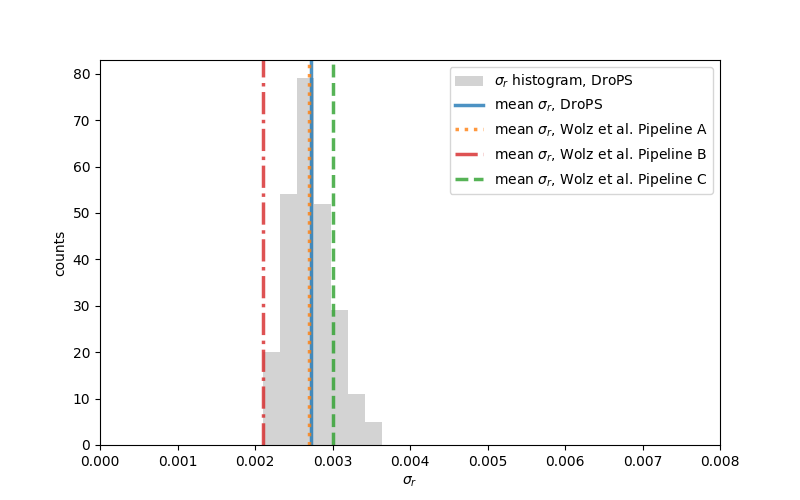
\includegraphics[width=0.5\textwidth]{dmsm_std.png}
  \caption{Comparing DroPS with three pipelines that are described in Wolf et al.~\cite{SO-SAT}. From top to bottom, foreground models ``d0, s0'', ``d1, s1'', and ``dm, sm'' are used, respectively. Left and right columns are the distrubution of reconstructed mean $r$ and $\sigma_r$, respectively.\label{fig:compare_SO}}
\end{figure}

\subsection{Map-level Operations}

The most well known method of component separation is probably the internal linear combination (ILC) algorithm and its variations. The basic idea is to isolate a signal - whose frequency dependence is known - by taking linear combination of the frequency maps. To do that in pixel space, the frequency maps have to be smoothed to a common resolution. 

For ground-based CMB experiments, however, a key challenge of ILC or ILC-like methods is that TOD filtering and beam convolution are non commutative operations. This prevents the frequency maps from being smoothed to a common resolution. Thus, while ILC remains popular in studies where the complexity of TOD filtering effect is ignored~\cite{SO-SAT}, likelihood-based method - which requires much more computing resources - has been used in real data analyses of BICEP/Keck~\cite{BKmap}.


The likelihood $\mathcal{L}\propto e^{-\chi^2/2}$ is based on a Gaussian noise model
\begin{equation}
  \chi^2 = \left(v_{\rm obs} - v_{\rm CMB} - v_{\rm FG}\right)^TN^{-1}\left(v_{\rm obs} - v_{\rm CMB} - v_{\rm FG}\right),
\end{equation}
where $v_{\rm obs}$ is the vector of observed frequency maps, $v_{\rm CMB}$ the CMB maps, $v_{\rm FG}$ the foreground maps, and $N$ the covariance of noise. In pixel space, the size of each vector is $n_{\rm pixel} n_{\rm frequency}$, i.e., product of the number of pixels and the number of frequency channels. For AliCPT or SO-SAT and maps with degree-scale resolution, we typically have $n_{\rm pixel} n_{\rm frequency} \gtrsim 10^4$. The number of elements in the covariance matrix $N$ is $\gtrsim 10^8$, which is difficult to estimate with simulations and also difficult to invert. The BICEP/Keck analysis~\cite{BKmap} only considers pixel auto-correlation, that is, the diagonal approximation of $N$.

\section{Technical Details}

\subsection{Foreground model}

The frequency dependence of dust temperature fluctuation is
\begin{equation}
  W_d(\nu) = \left(\frac{\nu}{\nu_{\rm ref}}\right)^{\beta_d-1}e^{\frac{h(\nu_{\rm ref} - \nu)}{k_BT_{\rm CMB}}}\left(\frac{e^{\frac{h\nu}{k_BT_{\rm CMB}}}-1}{e^{\frac{h\nu_{\rm ref}}{k_BT_{\rm CMB}}}-1}\right)^2 \left(\frac{e^{\frac{h\nu_{\rm ref}}{k_BT_{\rm MBB}}}-1}{e^{\frac{h\nu}{k_BT_{\rm MBB}}}-1}\right).
\end{equation}

The frequency dependence of synchrotron temperature fluctuation is
\begin{equation}
  W_s(\nu) = \left(\frac{\nu}{\nu_{\rm ref}}\right)^{\beta_s-2}e^{\frac{h(\nu_{\rm ref} - \nu)}{k_BT_{\rm CMB}}}\left(\frac{e^{\frac{h\nu}{k_BT_{\rm CMB}}}-1}{e^{\frac{h\nu_{\rm ref}}{k_BT_{\rm CMB}}}-1}\right)^2.
\end{equation}

\subsection{TOD filtering}

\bibliographystyle{unsrt}
\bibliography{refs} 

\end{document}
